\documentclass[12pt]{jsarticle}
\usepackage[dvipdfm,left=1.5cm,right=1.5cm,top=2cm]{geometry}
\usepackage[dvipdfmx]{graphicx}
\usepackage{amsmath, amssymb}
\usepackage{bm}
\usepackage{comment}
\usepackage{framed}
\usepackage{tabularx}

\setlength{\topmargin}{-1in}
\addtolength{\topmargin}{5mm}
\setlength{\headheight}{5mm}
\setlength{\headsep}{0mm}
\setlength{\textheight}{\paperheight}
\addtolength{\textheight}{-25mm}
\setlength{\footskip}{5mm}

\graphicspath{{image/}{image/box/}}

\newcommand{\frontpage}[3]{%
\begin{center}
 \\
\vspace{15em}{\LARGE{}レポート課題}\\
 \\
{\Huge\bf#1}\\
\vspace{30em}
{\LARGE\today}\\
\vspace{2em}
{\LARGE#2 #3}
\end{center}
\thispagestyle{empty}
\clearpage
\setcounter{page}{1}
}

\newcommand{\result}[5]{
\begin{minipage}{0.05\hsize}
(#1)
\end{minipage}
\begin{minipage}{0.22\hsize}
\includegraphics[width=\linewidth]{#2}j
\end{minipage}
\begin{minipage}{0.22\hsize}
\includegraphics[width=\linewidth]{#3}
\end{minipage}
\begin{minipage}{0.22\hsize}
\includegraphics[width=\linewidth]{#4}
\end{minipage}
\begin{minipage}{0.22\hsize}
\includegraphics[width=\linewidth]{#5}
\end{minipage}
\\
}

\begin{document}

\frontpage
{変分自己符号化器の特性評価}
{S152114}
{宮地 雄也}

\section{実験目的}

高精度な生成モデルとして有力視されている変分自己符号化器の原理および特性について理解する.

\section{実験原理}

\subsection{変分自己符号化器(Variational Autoencoder,VAE)}

変分自己符号化器について説明する.
以下の疑問に対する答えが含まれているようにすること.
\begin{itemize}
\item 再構成誤差および潜在誤差の定義とその意味.それぞれの数式が何を表しているか(特に$D_{KL}$の意味),および最小化することで何を達成しようとしているかがわかるようにすること.
\item 学習方法.演習課題を例に各パラメータの学習方法について数式を用いて具体的に説明すること.
\end{itemize}



**************************************


変分自己符号化器は自己符号化器とは異なり,潜在変数z(入力をエンコーダに通した値)に確率分布$N(0,1)$を仮定するというものである.
通常のオートエンコーダーは潜在変数にその特徴量をおし込めているが,変分オートエンコーダーは潜在変数を確率分布に$N(0,1)$と仮定することで,
よく似た形状のものを教師データがなくとも近い分布配置になる.
大まかなVAEのネットワークを図1に示す

\begin{figure}[ht]
  \begin{center}
    \includegraphics[width = 12cm]{VAE_image.png}
    \caption{VAEイメージ図}
  \end{center}
\end{figure}

VAEの構成は大きく分けて,古典的なAEと同じようにエンコーダー部分とデコーダー部分に分けることができる.
潜在変数にするまでがエンコーダー部分で,そこから画像に変換する部分がデコーダー部分に値する.
分散と平均から潜在確率を出力し,$D_{KL}$で精度を確認する.

今回,実験で使用したネットワーク構成を図2に示す.

\begin{figure}[ht]
  \begin{center}
    \includegraphics[width = 12cm]{VAE_detail.png}
    \caption{VAEイメージ図}
  \end{center}
\end{figure}

それぞれ計算は以下の通り.

\[
  \mu(x) = sigmoid (\sum_{i} (Wx+b))
\]

\[
  \sigma(x) = sigmoid ( \sum_{i} (Wx+b))
\]


\[
  z(x) = \mu(x)  + ( \sigma(x)+\epsilon)
\]




\clearpage
\section{実験方法}

今回実験では活性化層にいれる関数の性能評価を行う.
試す形式は,

\begin{enumerate}
    \item エンコーダー部分,デコーダー部分の活性化関数をすべてSigmoidに変更
  \begin{enumerate}
    \item 潜在変数の次元を2次元
    \item 潜在変数の次元を20次元
  \end{enumerate}
 \item エンコーダー部分,デコーダー部分の活性化関数をすべてReLUに変更
  \begin{enumerate}
    \item 潜在変数の次元を2次元
    \item 潜在変数の次元を20次元
  \end{enumerate}
\end{enumerate}



の二通りを潜在変数の次元を2次元と20次元の計4通りの実験を行う.ただし,$\mu$と$\sigma$は各次元に対して同一の構成で行う.


この4点について実験を行い、その効果を確認する.
上記のことを確認するために実験は次のように行う.

学習条件
\begin{itemize}
  \item 学習データ:MNISTデータセット
  \item 学習データ数:100枚
  \item テストデータ数;100枚
  \item 分類テストデータ数:1000枚
  \item 学習回数:2000回
  \item パラメーターの初期化方法:ガウス分布を0.1倍してランダムに初期化
  \item パラメータの更新方法:Adamアルゴリズムで更新
\end{itemize}


以下,詳細なネットワーク構成である.

\begin{table}[hbt]
\begin{center}
\caption{Encorder 1の構成(実験条件1-a)}
\label{table:Encorder1}
\begin{tabularx}{0.9\linewidth}{|l|l|X|}
\hline
1 & Affine層 & 入力ノード数:$784$,出力ノード数:$100$ \\
\hline
2 & 活性化層 & Sigmoid \\
\hline
3 & Affine層 & 入力ノード数:$100$,出力ノード数:$100$ \\
\hline
4 & 活性化層 & sigmoid \\
\hline
5 & Affine層 & 入力ノード数:$100$,出力ノード数:$2$ \\
\hline
\end{tabularx}
\end{center}
\end{table}


\begin{table}[hbt]
\begin{center}
\caption{Encorder 2の構成(実験条件2-a)}
\label{table:Encorder1}
\begin{tabularx}{0.9\linewidth}{|l|l|X|}
\hline
1 & Affine層 & 入力ノード数:$784$,出力ノード数:$100$ \\
\hline
2 & 活性化層 & ReLU \\
\hline
3 & Affine層 & 入力ノード数:$100$,出力ノード数:$100$ \\
\hline
4 & 活性化層 & ReLU \\
\hline
5 & Affine層 & 入力ノード数:$100$,出力ノード数:$2$ \\
\hline
\end{tabularx}
\end{center}
\end{table}

\begin{table}[hbt]
\begin{center}
\caption{Encorder 1の構成(実験条件1-b)}
\label{table:Encorder1}
\begin{tabularx}{0.9\linewidth}{|l|l|X|}
\hline
1 & Affine層 & 入力ノード数:$784$,出力ノード数:$100$ \\
\hline
2 & 活性化層 & Sigmoid \\
\hline
3 & Affine層 & 入力ノード数:$100$,出力ノード数:$100$ \\
\hline
4 & 活性化層 & sigmoid \\
\hline
5 & Affine層 & 入力ノード数:$100$,出力ノード数:$20$ \\
\hline
\end{tabularx}
\end{center}
\end{table}


\begin{table}[hbt]
\begin{center}
\caption{Encorder 2の構成(実験条件2-b)}
\label{table:Encorder1}
\begin{tabularx}{0.9\linewidth}{|l|l|X|}
\hline
1 & Affine層 & 入力ノード数:$784$,出力ノード数:$100$ \\
\hline
2 & 活性化層 & ReLU \\
\hline
3 & Affine層 & 入力ノード数:$100$,出力ノード数:$100$ \\
\hline
4 & 活性化層 & ReLU \\
\hline
5 & Affine層 & 入力ノード数:$100$,出力ノード数:$20$ \\
\hline
\end{tabularx}
\end{center}
\end{table}

\begin{table}[hbt]
\begin{center}
\caption{Encorder a μの構成(実験条件aは共通)}
\label{table:Encorder mu-1}
\begin{tabularx}{0.9\linewidth}{|l|l|X|}
\hline
1 & Affine層 & 入力ノード数:$2$,出力ノード数:$2$ \\
\hline
2 & 活性化層 & Sigmoid \\
\hline
\end{tabularx}
\end{center}
\end{table}

\begin{table}[hbt]
\begin{center}
\caption{Encorder a σの構成(実験条件aは共通)}
\label{table:Encorder sigma-1}
\begin{tabularx}{0.9\linewidth}{|l|l|X|}
\hline
1 & Affine層 & 入力ノード数:$2$,出力ノード数:$2$ \\
\hline
2 & 活性化層 & Sigmoid \\
\hline
\end{tabularx}
\end{center}
\end{table}


\begin{table}[hbt]
\begin{center}
\caption{Encorder b μの構成(実験条件bは共通)}
\label{table:Encorder mu-1}
\begin{tabularx}{0.9\linewidth}{|l|l|X|}
\hline
1 & Affine層 & 入力ノード数:$20$,出力ノード数:$20$ \\
\hline
2 & 活性化層 & Sigmoid \\
\hline
\end{tabularx}
\end{center}
\end{table}

\begin{table}[hbt]
\begin{center}
\caption{Encorder b σの構成(実験条件bは共通)}
\label{table:Encorder sigma-1}
\begin{tabularx}{0.9\linewidth}{|l|l|X|}
\hline
1 & Affine層 & 入力ノード数:$20$,出力ノード数:$20$ \\
\hline
2 & 活性化層 & Sigmoid \\
\hline
\end{tabularx}
\end{center}
\end{table}


\begin{table}[hbt]
\begin{center}
\caption{Decorde1 の構成(実験条件1-a)}
\label{table:Decorder}
\begin{tabularx}{0.9\linewidth}{|l|l|X|}
\hline
1 & Affine層 & 入力ノード数:$2$,出力ノード数:$100$ \\
\hline
2 & 活性化層 & Sigmoid \\
\hline
3 & Affine層 & 入力ノード数:$100$,出力ノード数:$100$ \\
\hline
4 & 活性化層 & Sigmoid \\
\hline
5 & Affine層 & 入力ノード数:$100$,出力ノード数:$100$ \\
\hline
6 & 活性化層 & Sigmoid \\
\hline
7 & Affine層 & 入力ノード数:$100$,出力ノード数:$784$ \\
\hline
8 & 活性化層 & Sigmoid \\
\hline

\end{tabularx}
\end{center}
\end{table}

\begin{table}[hbt]
\begin{center}
\caption{Decorde2 の構成(実験条件2-b)}
\label{table:Decorder}
\begin{tabularx}{0.9\linewidth}{|l|l|X|}
  \hline
  1 & Affine層 & 入力ノード数:$2$,出力ノード数:$100$ \\
  \hline
  2 & 活性化層 & ReLU \\
  \hline
  3 & Affine層 & 入力ノード数:$100$,出力ノード数:$100$ \\
  \hline
  4 & 活性化層 & ReLU \\
  \hline
  5 & Affine層 & 入力ノード数:$100$,出力ノード数:$100$ \\
  \hline
  6 & 活性化層 & ReLU \\
  \hline
  7 & Affine層 & 入力ノード数:$100$,出力ノード数:$784$ \\
  \hline
  8 & 活性化層 & Sigmoid \\
  \hline
\end{tabularx}
\end{center}
\end{table}



\begin{table}[hbt]
\begin{center}
\caption{Decorde1 の構成(実験条件2-a)}
\label{table:Decorder}
\begin{tabularx}{0.9\linewidth}{|l|l|X|}
\hline
1 & Affine層 & 入力ノード数:$20$,出力ノード数:$100$ \\
\hline
2 & 活性化層 & Sigmoid \\
\hline
3 & Affine層 & 入力ノード数:$100$,出力ノード数:$100$ \\
\hline
4 & 活性化層 & Sigmoid \\
\hline
5 & Affine層 & 入力ノード数:$100$,出力ノード数:$100$ \\
\hline
6 & 活性化層 & Sigmoid \\
\hline
7 & Affine層 & 入力ノード数:$100$,出力ノード数:$784$ \\
\hline
8 & 活性化層 & Sigmoid \\
\hline

\end{tabularx}
\end{center}
\end{table}
\clearpage

\begin{table}[hbt]
\begin{center}
\caption{Decorde2 の構成(実験条件2-b)}
\label{table:Decorder}
\begin{tabularx}{0.9\linewidth}{|l|l|X|}
  \hline
  1 & Affine層 & 入力ノード数:$20$,出力ノード数:$100$ \\
  \hline
  2 & 活性化層 & ReLU \\
  \hline
  3 & Affine層 & 入力ノード数:$100$,出力ノード数:$100$ \\
  \hline
  4 & 活性化層 & ReLU \\
  \hline
  5 & Affine層 & 入力ノード数:$100$,出力ノード数:$100$ \\
  \hline
  6 & 活性化層 & ReLU \\
  \hline
  7 & Affine層 & 入力ノード数:$100$,出力ノード数:$784$ \\
  \hline
  8 & 活性化層 & Sigmoid \\
  \hline
\end{tabularx}
\end{center}
\end{table}





\subsection{自己符号化器の再構成精度および入力分布と出力分布の対応}

再構成精度が高くなるように自己符号化器を設計し,学習を行う.
学習の進行状況を確認するために,学習データおよびテストデータに対する再構成誤差および潜在誤差の変化を表すグラフを作成する.
また,学習結果を確認するために,学習データおよびテストデータに対する復号化器の出力を画像化する.
加えて,入力した学習データの分布と出力された復号画像の分布を比較するために,
画像中の適当な位置を数点選択し,度数分布図を作成する.

再構成誤差には二乗和誤差およびクロスエントロピーを用い比較した.



\subsection{潜在変数の分布と出力分布の対応}

$z$の値を(-2,-2)から(2,2)まで変化させ,復号化器の出力を画像化する.出力画像はzの平面上の位置関係を保つように並べること.
異なる数字の学習データの組$x_1$および$x_2$に対応する潜在変数$z_1$および$z_2$の線形結合$z=t z_1+(1-t) z_2$における$t$の値を1から0まで変化させ,
復号化器の出力を画像化する.出力画像は$t$の直線上の位置関係を保つように並べる.



\section{実験結果}

実験結果は以下のとおりである.


\begin{figure}[ht]
  \begin{center}
    \begin{tabular}{c}

      % 1
      \begin{minipage}{0.5\hsize}
        \begin{center}
          \includegraphics[clip, width=\linewidth]{sig_final_train_mode_z2_1_1999.png}
          \hspace{0.2cm} 実験1-a (活性化関数:Sigmoid)
        \end{center}
      \end{minipage}

      % 2
      \begin{minipage}{0.5\hsize}
        \begin{center}
          \includegraphics[clip, width=\linewidth]{ReLU_final_train_mode_z20_2_1999.png}
          \hspace{0.2cm} 実験1-b (活性化関数:ReLU)
        \end{center}
      \end{minipage}\\\\

      % 3
      \begin{minipage}{0.5\hsize}
        \begin{center}
          \includegraphics[clip, width=\linewidth]{sig_final_train_mode_z20_1_1999.png}
          \hspace{0.2cm} 実験2-a (活性化関数:Sigmoid)
        \end{center}
      \end{minipage}

      % 4
      \begin{minipage}{0.5\hsize}
        \begin{center}
          \includegraphics[clip, width=\linewidth]{ReLU_inal_train_mode_z2_2_1999.png}
          \hspace{0.2cm} 実験2-b (活性化関数:ReLU)
        \end{center}
      \end{minipage}

    \end{tabular}
    \caption{出力画像}
     \label{fig:output2}
  \end{center}
\end{figure}

\begin{figure}[ht]
  \begin{center}
    \begin{tabular}{c}

      % 1
      \begin{minipage}{0.5\hsize}
        \begin{center}
          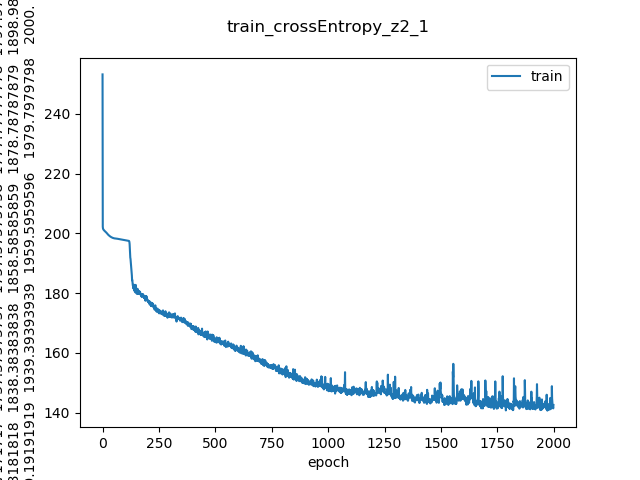
\includegraphics[clip, width=\linewidth]{plottrain_crossEntropy_z2_1.png}
          \hspace{0.2cm} 実験1-a (活性化関数:Sigmoid)
        \end{center}
      \end{minipage}

      % 2
      \begin{minipage}{0.5\hsize}
        \begin{center}
          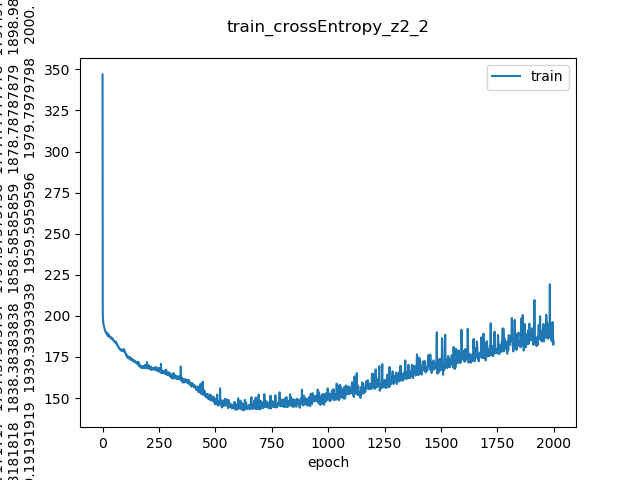
\includegraphics[clip, width=\linewidth]{plottrain_crossEntropy_z2_2.png}
          \hspace{0.2cm} 実験1-b (活性化関数:ReLU)
        \end{center}
      \end{minipage}\\\\

      % 3
      \begin{minipage}{0.5\hsize}
        \begin{center}
          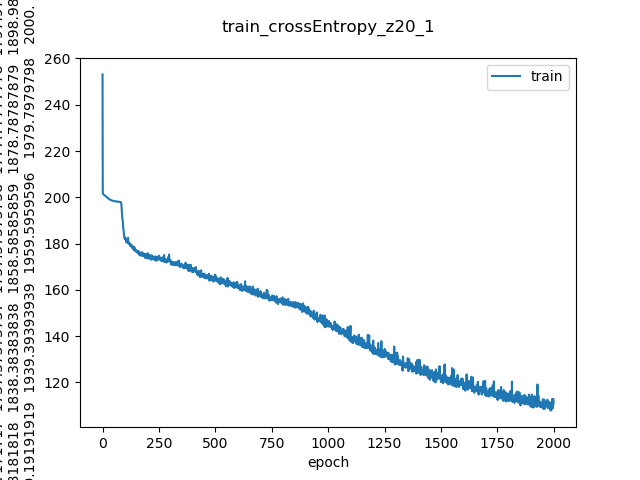
\includegraphics[clip, width=\linewidth]{plottrain_crossEntropy_z20_1.png}
          \hspace{0.2cm} 実験2-a (活性化関数:Sigmoid)
        \end{center}
      \end{minipage}

      % 4
      \begin{minipage}{0.5\hsize}
        \begin{center}
          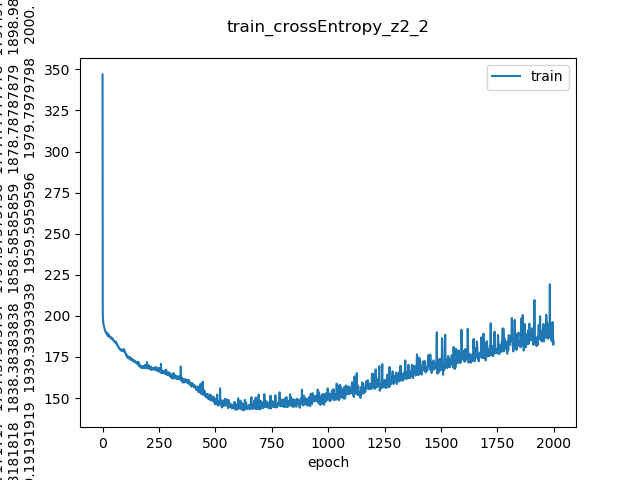
\includegraphics[clip, width=\linewidth]{plottrain_crossEntropy_z2_2.png}
          \hspace{0.2cm} 実験2-b (活性化関数:ReLU)
        \end{center}
      \end{minipage}

    \end{tabular}
    \caption{crossEntorpy}
     \label{fig:crossEntorpy2}
  \end{center}
\end{figure}



\begin{figure}[ht]
  \begin{center}
    \begin{tabular}{c}

      % 1
      \begin{minipage}{0.5\hsize}
        \begin{center}
          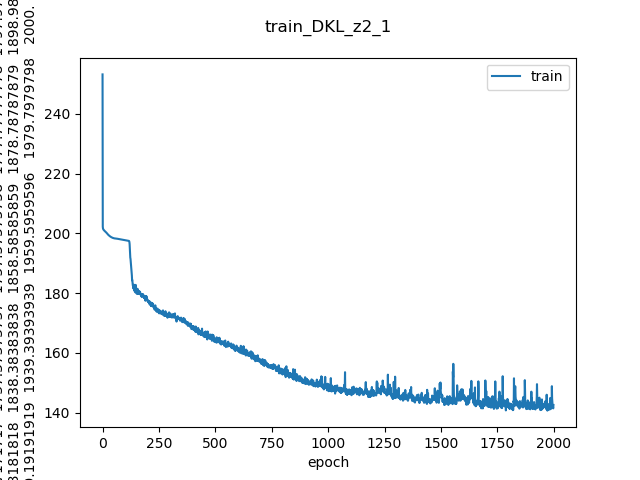
\includegraphics[clip, width=\linewidth]{plottrain_DKL_z2_1.png}
          \hspace{0.2cm} 実験1-a (活性化関数:Sigmoid)
        \end{center}
      \end{minipage}

      % 2
      \begin{minipage}{0.5\hsize}
        \begin{center}
          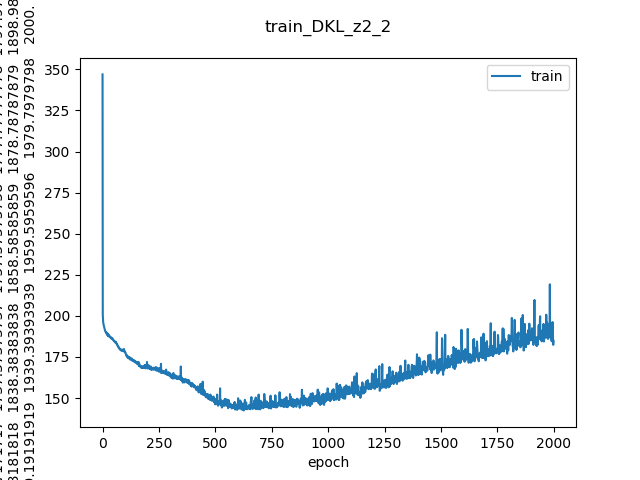
\includegraphics[clip, width=\linewidth]{plottrain_DKL_z2_2.png}
        \hspace{0.2cm} 実験1-b (活性化関数:ReLU)
        \end{center}
      \end{minipage}\\\\

      % 3
      \begin{minipage}{0.5\hsize}
        \begin{center}
          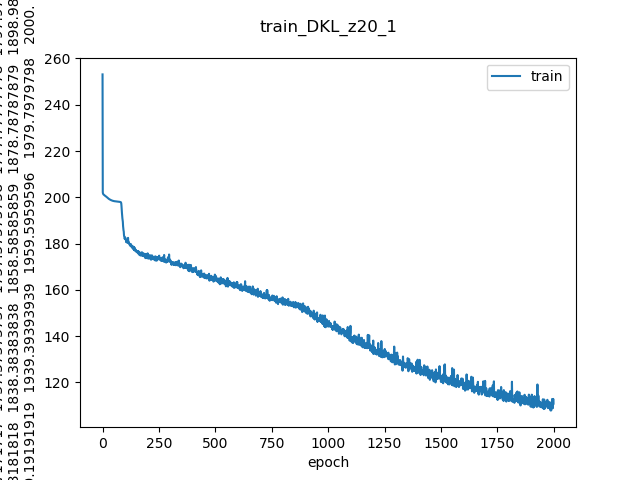
\includegraphics[clip, width=\linewidth]{plottrain_DKL_z20_1.png}
          \hspace{0.2cm} 実験2-a (活性化関数:Sigmoid)
        \end{center}
      \end{minipage}

      % 4
      \begin{minipage}{0.5\hsize}
        \begin{center}
          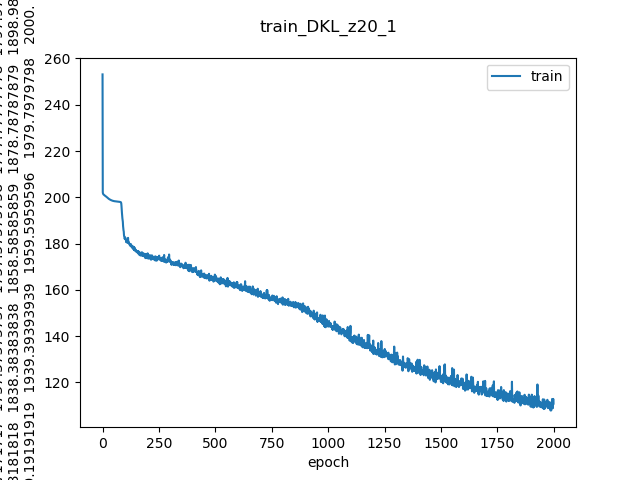
\includegraphics[clip, width=\linewidth]{plottrain_DKL_z20_1.png}
          \hspace{0.2cm} 実験2-b (活性化関数:ReLU)
        \end{center}
      \end{minipage}

    \end{tabular}
    \caption{$D_{KL}$}
     \label{fig:DKL2}
  \end{center}
\end{figure}


\begin{figure}[ht]
  \begin{center}
    \begin{tabular}{c}

      % 1
      \begin{minipage}{0.5\hsize}
        \begin{center}
          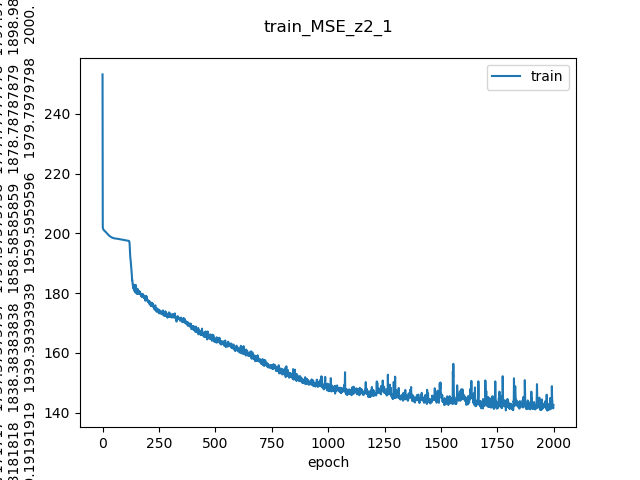
\includegraphics[clip, width=\linewidth]{plottrain_MSE_z2_1.png}
          \hspace{0.2cm} 実験1-a (活性化関数:Sigmoid)
        \end{center}
      \end{minipage}

      % 2
      \begin{minipage}{0.5\hsize}
        \begin{center}
          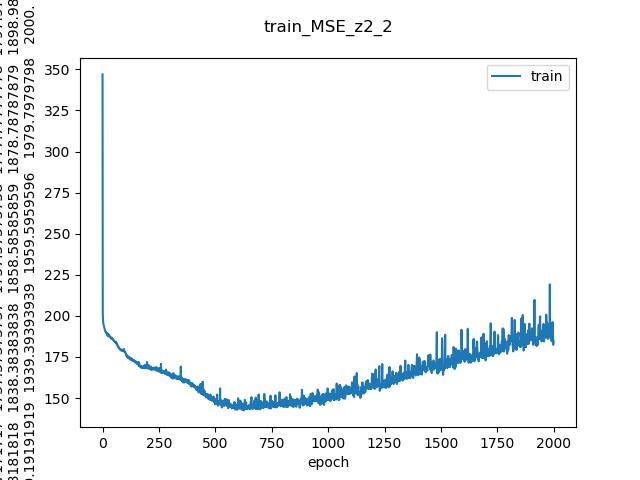
\includegraphics[clip, width=\linewidth]{plottrain_MSE_z2_2.png}
        \hspace{0.2cm} 実験1-b (活性化関数:ReLU)
        \end{center}
      \end{minipage}\\\\


      % 3
      \begin{minipage}{0.5\hsize}
        \begin{center}
          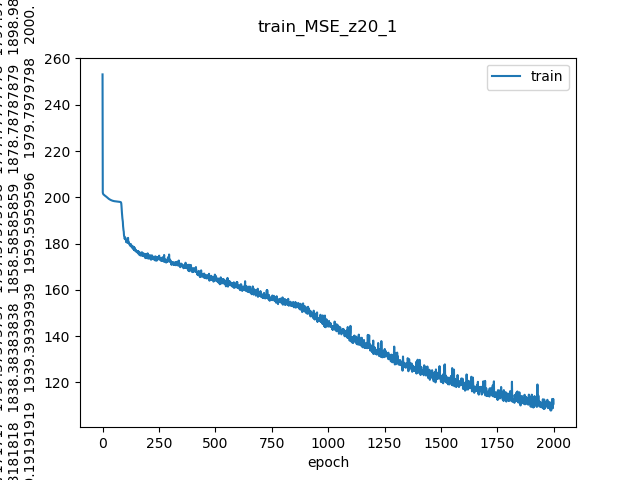
\includegraphics[clip, width=\linewidth]{plottrain_MSE_z20_1.png}
          \hspace{0.2cm} 実験2-a (活性化関数:Sigmoid)
        \end{center}
      \end{minipage}

      % 4
      \begin{minipage}{0.5\hsize}
        \begin{center}
          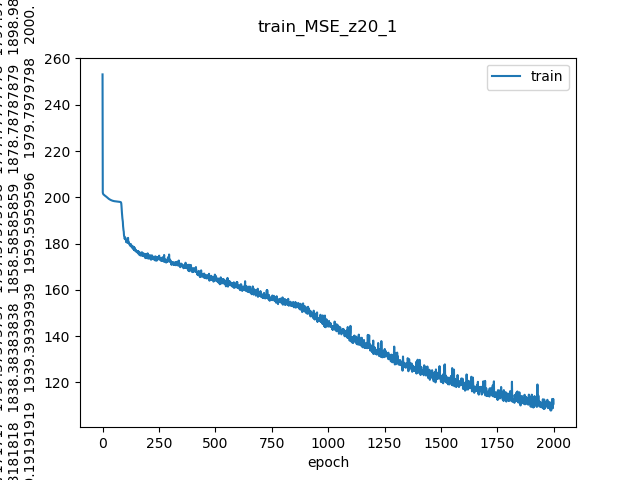
\includegraphics[clip, width=\linewidth]{plottrain_MSE_z20_1.png}
          \hspace{0.2cm} 実験2-b (活性化関数:ReLU)
        \end{center}
      \end{minipage}

    \end{tabular}
    \caption{平均二乗誤差}
     \label{fig:MSE2}
  \end{center}
\end{figure}


\begin{figure}[ht]
  \begin{center}
    \begin{tabular}{c}

      % 1
      \begin{minipage}{0.5\hsize}
        \begin{center}
        \includegraphics[clip, width=\linewidth]{zdata_z2_1.png}
        \hspace{0.2cm} 実験1-a (活性化関数:Sigmoid)
        \end{center}
      \end{minipage}

      % 2
      \begin{minipage}{0.5\hsize}
        \begin{center}
        \includegraphics[clip, width=\linewidth]{zdata_z2_2.png}
        \hspace{0.2cm} 実験1-b (活性化関数:ReLU)
        \end{center}
      \end{minipage}\\\\


      % 3
      \begin{minipage}{0.5\hsize}
        \begin{center}
          \includegraphics[clip, width=\linewidth]{zdata_z20_1.png}
          \hspace{0.2cm} 実験2-a (活性化関数:Sigmoid)
        \end{center}
      \end{minipage}

      % 4
      \begin{minipage}{0.5\hsize}
        \begin{center}
          \includegraphics[clip, width=\linewidth]{zdata_z20_2.png}
          \hspace{0.2cm} 実験2-b (活性化関数:ReLU)
        \end{center}
      \end{minipage}

    \end{tabular}
    \caption{散布図}
     \label{fig:sannpu2}
  \end{center}
\end{figure}





\section{考察}

実験結果をもとに,再構成精度を高める上で重要と考えられる要因について分析する.また,入力および出力分布の比較結果について考察する.

潜在変数の分布をもとに,各数字の潜在空間における位置関係の意味について検討する.潜在変数の次元の違いによる影響についても考察すること.

\end{document}
